
\documentclass[runningheads,a4paper]{llncs}
\usepackage[margin=0.5in]{geometry}
\usepackage{amssymb}
\setcounter{tocdepth}{3}
\usepackage{graphicx}
\usepackage{amssymb}% http://ctan.org/pkg/amssymb
\usepackage{pifont}% http://ctan.org/pkg/pifont
\newcommand{\cmark}{\ding{51}}%
\newcommand{\xmark}{\ding{55}}%

\usepackage{floatrow}
% Table float box with bottom caption, box width adjusted to content
\newfloatcommand{capbtabbox}{table}[][\FBwidth]
\usepackage{caption}
\usepackage{subcaption}
\captionsetup{compatibility=false}

\usepackage{url} % for bibliograpy links
\urlstyle{same}  % (for bibliography links
\usepackage{float} % To force image to stand still

\usepackage{amsmath,amssymb}

\usepackage{color}

\usepackage{array}
\newcolumntype{P}[1]{>{\centering\arraybackslash}p{#1}}

\newcommand{\keywords}[1]{\par\addvspace\baselineskip
\noindent\keywordname\enspace\ignorespaces#1}

\begin{document}
\vspace{-100pt}
\mainmatter

\title{A Stochastic Approach to Optimization of Deterministic Finite Automata}

\titlerunning{Algorithms and Computability}

\author{Jakub Ciecierski \and Bartlomiej Dybisz \\ 
\textit{Warsaw University of Technology,\\
Faculty of Mathematics and Information Science.}}

\authorrunning{Algorithms and Computability}


\toctitle{Algorithms and Computability}
\tocauthor{Methodology}

\maketitle



%---------------------------------------------------------------------
%---------------------------------------------------------------------
\section{Change Log}\label{sec:algorithm}

\subsubsection{PSO Particle Interval}

The position of our particles will be represented by the natural decoding vector of size $n*r$ of an automaton described in the methodology with more freedom allowed. Namely, all of the dimensions of the position will take real values in the interval $[0.5, (n+0.5)]$. Whenever we need to encode the automaton back, we simply round up the values, taking the closest integer value. The real number $3.4$ becomes $3$ and $3.5$ becomes 4. Notice that the interval is expanded by the value $0.5$. Such procedure is needed to allow for equal distribution of the first and last states. Namely, the first state will be encoded for values: $[0.5, 1.5]$ and the last state: $[(n-0.5), (n+0.5)]$.

\subsubsection{PSO Particle Update}

We added another method of updating particles. Instead of PSO11 particle update we process the particle moving algorithm with legacy approach of PSO from 1995. The experiments showed better result in the fallowing approach.

\begin{equation}
		V_p(t+1) = V_p(t) + c_1 * \mu_1 *(pbest_p - X_p(t)) + c_2 * \mu_2 *(lbest_p - X_p(t))
	\end{equation}

	\begin{equation}
		X_p(t+1) = X_p(t) + V_p(t)
	\end{equation}
	where:\\
	$c_1, c_2$ are the constant learning factors.\\
	$\mu_1, \mu_2$ are random numbers in the range [0,1].



%---------------------------------------------------------------------
\section{Console}

The following figure presents the example of console application.

\begin{figure}[H]
	\centering
	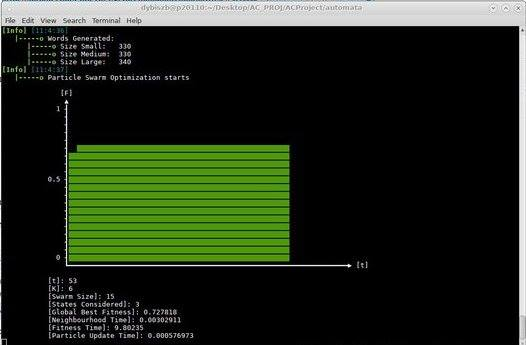
\includegraphics[width=0.6\textwidth]{images/console.jpg}
    \caption{Example of console}
    \label{fig:clustering_class}
\end{figure}

\end{document}
